\section{Weryfikacja rozwiązania}
W celu skorzystania z programu agilemaster, należy stworzyć wspomniane wcześniej pliki z danymi użytkownika oraz danymi dostępowymi do api.
Następnie, wprowadzamy do programu wybrane parametry. Nazwa projektu musi zgadzać się z nazwą projektu stworzonego na instancji Jiry, podobnie jak nazwy statusów.
Kolejność podania statusów ma znaczenie, ponieważ bez dodatkowej konfiguracji nie jest możliwy inny sposób ustalenia ich naturalnej progresji.
\begin{lstlisting}[caption=Przykładowe użycie programu agilemaster]
PS C:\Users\Kuba\RustroverProjects\agilemaster> agilemaster `
>> --name kanban-test `
>> --author user.json `
>> --auth auth.json `
>> --start 01-02-2024 `
>> --end 31-03-2024 `
>> --issues 70 `
>> --statuses "BACKLOG" "SELECTED FOR DEVELOPMENT" "IN PROGRESS" "DONE"
\end{lstlisting}

W efekcie takiego wywołania tworzony jest plik \texttt{kanban-test.json} (nazwa wygenerowana na podstawie podanej nazwy projektu).
Należy stworzyć pusty projekt typu Kanban, a następnie na swojej instancji Jiry w ustawieniach wybrać kategorię "System", a następnie zakładkę "External System Import".
Należy zwrócić uwagę że w przypadku wyboru konfiguracji "Team-managed" i "Company-managed" w projekcie domyślnie mamy dostępne inne statusy.
Statusy w projekcie można dowolnie dostosować, pamiętając jednak aby poprawnie podać je przy użyciu programu agilemaster.
\begin{figure}[H]
    \centering
    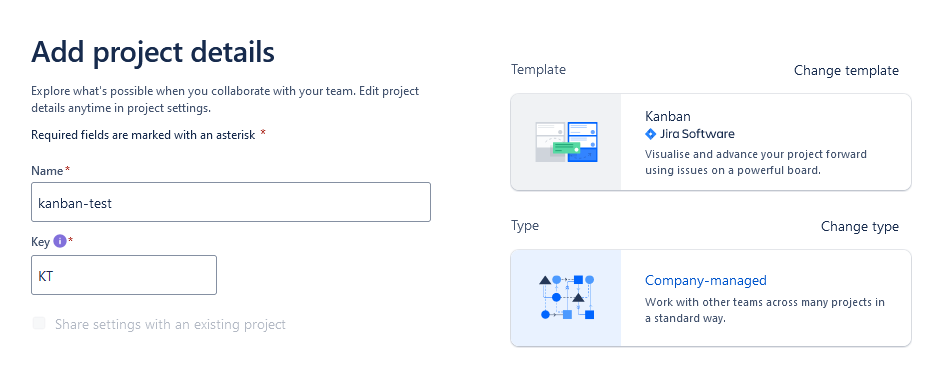
\includegraphics[width=15cm,keepaspectratio]{rysunki/jira-create-project.png}
    \caption{Tworzenie projektu Kanban w konfiguracji Company-managed}
\end{figure}

\begin{figure}[H]
    \centering
    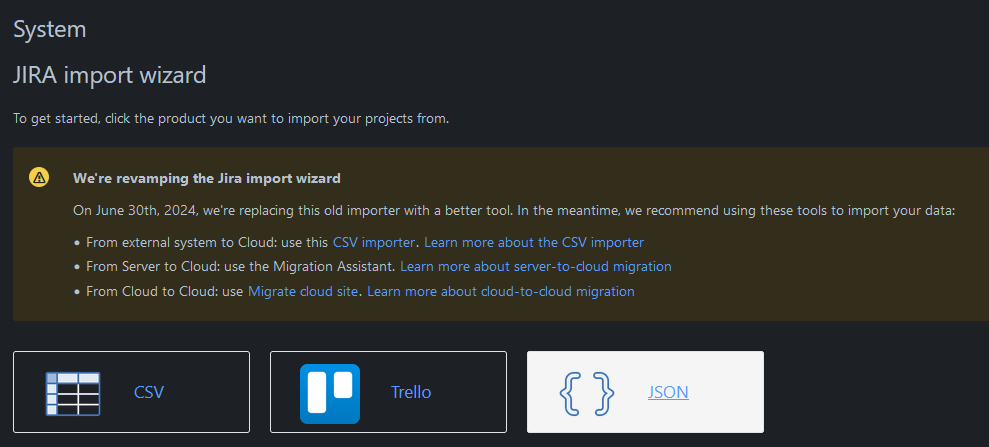
\includegraphics[width=15cm,keepaspectratio]{rysunki/jira-import-wizard.png}
    \caption{Narzędzie do importu danych na Jirę}
\end{figure}

Po pomyślnym zakończeniu importu danych, wszystkie zadania możemy zaobserwować w projekcie.
\begin{figure}[H]
    \centering
    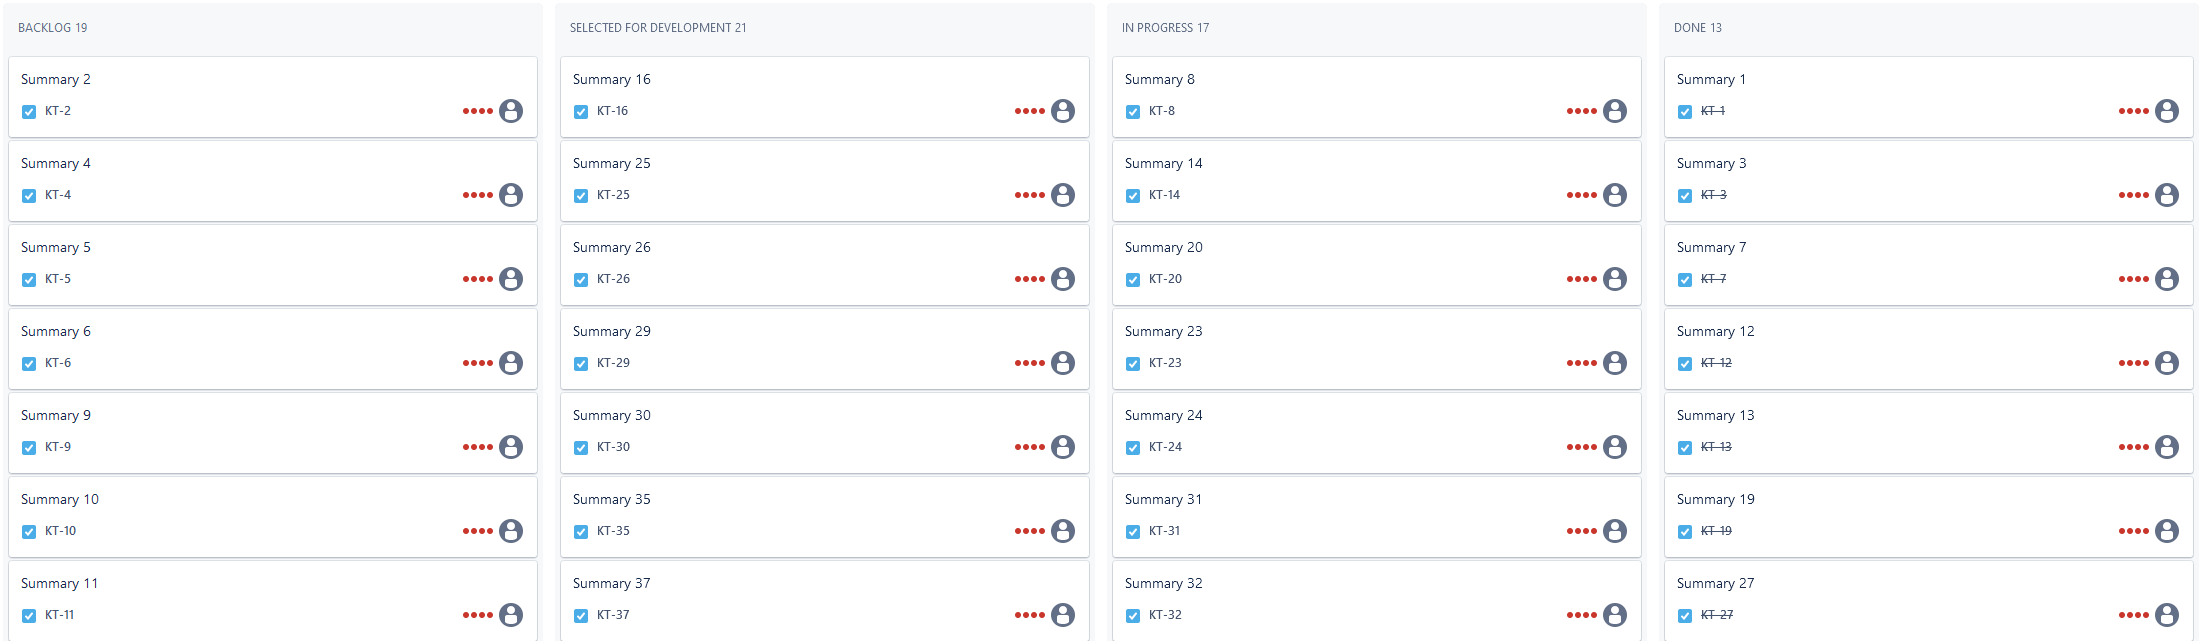
\includegraphics[width=15cm,keepaspectratio]{rysunki/jira-board.png}
    \caption{Fragement tablicy wypełnionej zaimportowanymi zadaniami}
\end{figure}

Przy inspekcji zakładki "History" w zadaniu możemy zaobserwować poprawną chronologię w zmianach statusów.
\begin{figure}[H]
    \centering
    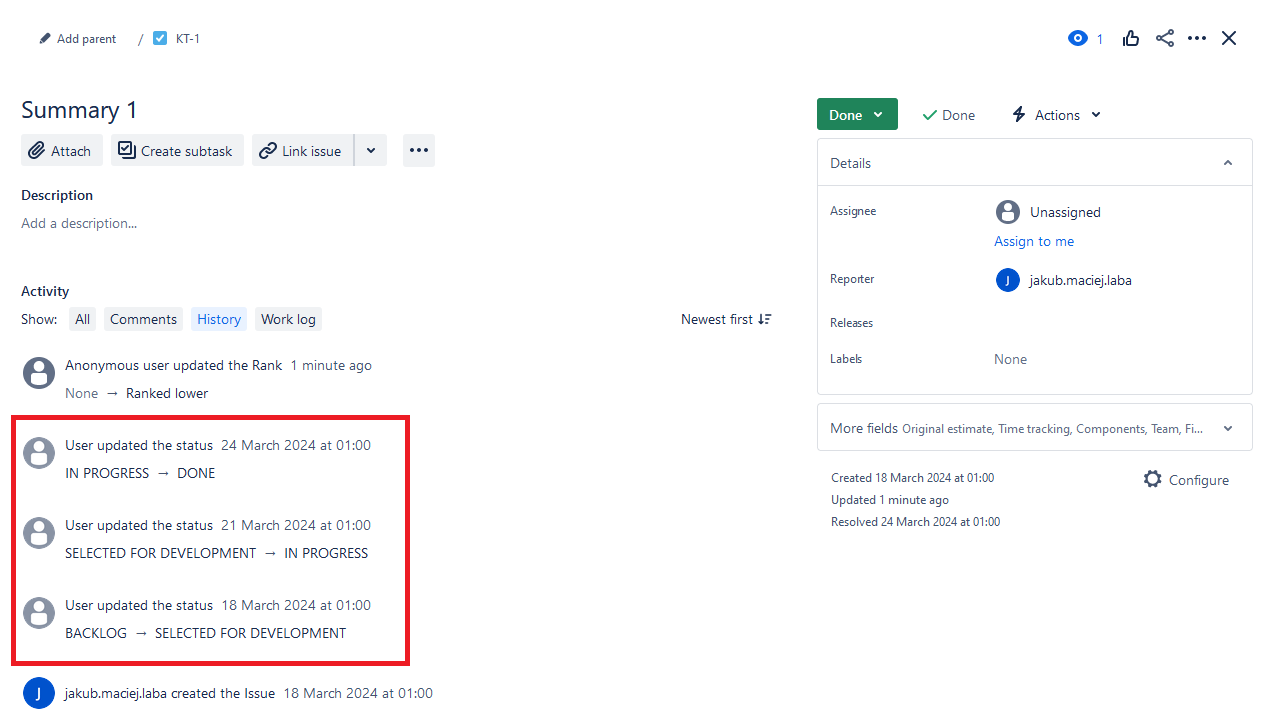
\includegraphics[width=15cm,keepaspectratio]{rysunki/jira-issue-history.png}
    \caption{Historia przykładowego zaimportowanego zadania}
\end{figure}
